% Kepler Conjecture.
% Thomas C. Hales
% Starting with Chapter on Tame Hypermaps


%% XX Notation: A vs. v for nodes.
%% XX Notation sigma' for aggregates, sigma'' for the full hypermap.
%% Allow the pentagon-triangle into the definition of tame graph.
%%%% Show there is at most one.  Let it be the seed.
%%




\label{sec:tame}


This chapter defines a class of hypermaps.  Hypermaps in this class
are said to be {\it tame}.  In the next chapter, we give a complete
classification of all tame hypermaps.  This classification of tame
hypermaps was carried out by computer.   This classification is a
major step of the proof of the Kepler Conjecture.

\section{Basic Definitions}


\begin{definition}
Faces of cardinality $3$ are called {\it triangles}, those of
cardinality $4$ are called {\it quadrilaterals}, and so forth. Let
$p_v$ be the number of triangles incident with a node $v$. A face of
cardinality at least $5$ is called an {\it exceptional\/} face.
 %
 \index{triangle}
 \index{exceptional}
 \index{quadrilateral}
 \index{exceptional!face}
 \index{pZ@$p_v$}
\end{definition}

\begin{definition}\label{definition:type}
A face of a hypermap is said to be exceptional if it has at least
five darts.  The {\it type\/} of a node is defined to be a triple of
non-negative integers $(p,q,r)$, where $p$ is the number of
triangles containing the node, $q$ is the number of quadrilaterals
containing it, and $r$ is the number of exceptional faces.
%
 \index{type (of a node)}
\end{definition}


\section{Weight Assignments}\label{sec:wtassign}

We call the constant $\op{tgt}=14.8$, which arises repeatedly in
this section, the {\it target}.  (This constant arises as an
approximation to $4\pi\zeta -8\approx 14.7947$, where $\zeta =
1/(2\arctan(\sqrt{2}/5)$.)
%
 \index{target}\index{tgt@$\op{tgt}=14.8$}
 \index{ZZdzeta@$\zeta= 1/(2\arctan(\sqrt{2}/5))$}

\begin{definition}
  Define $a:\ring{N}\to \ring{R}$ by
  $$a(n) = \begin{cases}
    14.8 &n=0,1,2,\\
    1.4 & n=3,\\
    1.5 & n=4,\\
    0 & \text{otherwise.}
  \end{cases}
  $$
\end{definition}

\begin{definition}
  Define $b:\ring{N}\times \ring{N}\to \ring{R}$ by $b(p,q)=14.8$,
  except for the values in the following table
  (with  $\op{tgt}=14.8$):
  {
  \def\tx{\op{tgt}}
  $$\begin{matrix}  &q=0&1&2&3&4\\
           p=0&\tx&\tx&\tx&7.135&10.649\\
           1&\tx&\tx&6.95&7.135&\tx\\
           2&\tx&8.5&4.756&12.981&\tx\\
           3&\tx&3.642&8.334&\tx&\tx\\
           4&4.139&3.781&\tx&\tx&\tx\\
           5&0.55&11.22&\tx&\tx&\tx\\
           6&6.339&\tx&\tx&\tx&\tx
   \end{matrix}
   $$
   }
\end{definition}

\begin{definition}
  Define $c:\ring{N}\to \ring{R}$ by
  $$c(n) = \begin{cases}
    1 & n=3,\\
    0 & n=4,\\
    -1.03 &n=5,\\
    -2.06 &n=6,\\
    -3.03 &\text{otherwise.}
    \end{cases}
    $$
\end{definition}

\begin{definition}
    Define $d:\ring{N}\to \ring{R}$ by
  $$d(n) = \begin{cases}
    0 & n=3, \\
    2.378 & n=4, \\
    4.896 & n=5, \\
    7.414 & n=6, \\
    9.932 & n=7, \\
    10.916 & n=8,\\
    \op{tgt}=14.8 & \text{otherwise}.
  \end{cases}
  $$
\end{definition}

\begin{definition}
A set $V$ of nodes in a hypermap is called a {\it separated\/} set
of nodes if the following four conditions hold.
%
 \index{separated set}
    \begin{enumerate}
      \item Every node in $V$ is incident with an exceptional face.
      \item No two
        nodes in $V$ are adjacent.  (That is, no edge is incident
        with two different nodes in $V$.)
      \item No quadrilateral in $V$ is incident with two different nodes
        in $V$.
      \item Each node in $V$ has cardinality 5.
    \end{enumerate}
\end{definition}

\begin{definition}
%
A {\it weight assignment\/} of a hypermap $H$ is a function $w$ on
the set of faces of $H$, taking values in the set of non-negative
real numbers. A weight assignment is {\it admissible} if the
following properties hold:
%
 \index{weight assignment}
 \index{admissible (weight assignment)}
\begin{enumerate}
  \item If the face $F$ has cardinality $n$, then
        $w(F) \ge d(n)$
  \item If a node $v$ has type $(p,q,0)$, then
        $$\sum_{F:\,v\cap F\ne\emptyset} w(F) \ge b(p,q).$$
        \label{admissible:b}
  \item Let $V$ be any set of nodes of type $(5,0,0)$, and let $A =\bigcup V$ be
        the set of darts in these nodes.
        If the cardinality of $V$ is $k\le 4$, then
        then
        $$\sum_{F:\,F\cap A\ne\emptyset} w(F) \ge 0.55 k.$$
  \item Let $V$ be any separated set of nodes, and let $A =\bigcup V$ be
        the set of darts in these nodes.
        Then
        $$\sum_{F:\,F\cap A\ne\emptyset} (w(F) -d(\card(F)))
            \ge \sum_{v\in V} a(p_v).$$
        \label{definition:admissible:excess}
\end{enumerate}
The sum $\sum_F w(F)$ is called the {\it total weight} of $w$.
\index{total weight}
\end{definition}





\section{Hypermap Properties}
\label{sec:graphproperty}

We say that a hypermap is {\it tame\/} if it satisfies the following
conditions.
%
 \index{tame}

\begin{enumerate}
    \label{definition:tame}
    %1
    \item The hypermap is plain, planar, and connected.
    \item The edge map $e$ has no fixed points.
    \item The two darts of each edge lie in different nodes.
    \item The set of edges meeting any two given nodes has cardinality at most $1$.
    \item There are at least $2$ faces.
    \item Every face meets every node in at most one
        dart.
    \item There are never two nodes of type $(4,0,0)$ that are
    adjacent to each other.
    \label{definition:tame:40}
    \item The cardinality of each face is at least $3$ and at most $8$.
    \label{definition:tame:length}

    \item If $L$ is a contour loop with $3$ face steps, and if there exists a node in
    the exterior of $L$, then $L$ is a face of the hypermap.
    \label{definition:tame:3-circuit}

    \item If $L$ is a contour loop  $4$ face steps, and there are at least two nodes
    in the exterior of $L$, then the interior of $L$ takes one of the forms
    illustrated in Figure
    \ref{fig:fourcircuit}.  [XX make this more precise.]
    \label{definition:tame:4-circuit}
    \begin{figure}[htb]
        \centering
        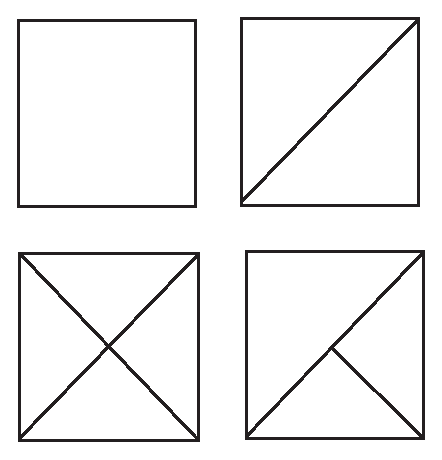
\includegraphics{\ps/tame4circuit.eps}
        \caption{Tame $4$-circuits}
        \label{fig:fourcircuit}
    \end{figure}

    \item The cardinality of every node is at least $2$ and at most
    $6$.
    \label{definition:tame:degree}

    \item If a node is incident with an exceptional face,
        then the cardinality of the node is at most $5$.
    \label{definition:tame:degreeE}

    \item $$\sum_F c(\card(F)) \ge 8,$$
    \label{definition:tame:score}


    \item There exists an admissible weight assignment
        of total weight less than the target, $\op{tgt}=14.8$.
    \label{definition:tame:squander}



\end{enumerate}
%
Property \ref{definition:tame:score} implies that the hypermap has
at least eight triangles.


\chapter{Classification of Tame Hypermaps}
    \label{sec:proof-classification}

\section{Statement of the Theorem}
\label{sec:classification}

A list of several thousand hypermaps appears at \cite{web}. The
following theorem is listed as one of the central claims in the
proof in Section~\ref{sec:logic}.

\begin{definition} The opposite of a hypermap $(D,e,n,f)$ is the
hypermap $(D,f n,n^{-1},f^{-1})$.
\end{definition}

\begin{lemma} If a hypermap has properties XXX, then so does its
opposite.
\end{lemma}

\begin{theorem}
\label{theorem:classification} Every tame hypermap is isomorphic to
a hypermap in this list, or is isomorphic to the opposite of a
hypermap in this list.
\end{theorem}

The results of this section are not needed except in the proof of
Theorem \ref{theorem:classification}.

\smallskip

Computers are used to generate a list of all hypermaps and to check
them against the archive of tame hypermaps.  The computer program is
based on the face-insertion construction of Lemma~XX.  There it is
proved that all sufficiently nice hypermaps can be generated by an
elementary face-insertion process.  Tame hypermaps satisfy all the
hypotheses of that lemma.



\chapter{Formally Contravening Hypermaps}
    \label{sec:startame}

In this chapter we consider tuples $(H,\azim,\flat,\sigma)$, where
$H$ is a hypermap, $\azim$ is real-valued function on the darts of
$H$, $\flat$ is a  boolean valued function on a subset of the darts,
and $\sigma$ is a real-valued function on its set of faces. We will
define a formally contravening hypermap to be a tuple
$(H,\azim,\flat,\sigma)$ satisfying a long list of conditions. The
main result of this chapter (Theorem~\ref{theorem:contravene}) will
be that if the pair $(H,\azim,\flat,\sigma)$ satisfies this long
list of conditions, then $H$ must be a tame hypermap.

The function $\azim$ will be an abstract version of the azimuth
function that appears in SectionXX.  The function $\flat$ is an
abstraction of the assertion that there is a flat quarter at $x$.
Similarly, the function $\sigma$ is an abstraction of the scoring
function that appears in Section XX. However, we will be careful not
to use any properties of $\azim$ and $\sigma$ other than those
explicitly stated as part of the definition of formally contravening
hypermap. This chapter is entirely formal in the sense that no
vectors, Euclidean geometry, or measure theory will make an
appearance.  The chapter does rely heavily on properties of
hypermaps.  By abuse of notation, we will sometimes refer to $H$ as
the formally contravening hypermap.

\begin{definition}  Lemmas XX state various properties of tuples
$(H,\azim,\flat,\sigma)$.  We define a {\it formally contravening
hypermap\/} to be any tuple $(H,\azim,\flat,\sigma)$ that satisfy
these properties.  (Thus, Lemmas XX are all tautologically true by
virtue of this definition; and nothing further can be concluded
about formally contravening hypermaps, except for facts deduced from
these lemmas.)
\end{definition}

\begin{theorem} \label{theorem:contravene}
Let $(H,\azim,\flat,\sigma)$ be a formally contravening hypermap.
Then $H$ is a tame hypermap.
\end{theorem}

Recall that we say that a node $v$ has {\it type\/} $(p,q,r)$ if
there are exactly $p+q+r$ faces that meet the node, of which exactly
$p$ triangles and $q$ quadrilateral faces (see
Definition~\ref{definition:type}).  We write $(p_v,q_v,r_v)$ for the
type of a node $v$.



\begin{lemma}  Let $(H,\azim,\flat,\sigma)$ be a formally contravening
hypermap.  The hypermap $H$ satisfies Conditions XX-XX of tameness.
Explicitly, it is a plain, planar, and connected. The edge map $e$
has no fixed points. There are at least two faces. Every face meets
every node in at most one dart.  There are never two nodes of type
$(4,0,0)$ that are adjacent to each other.  Every face has
cardinality at least $3$ and at most $8$.  If $L$ is a contour loop
with $3$ face steps, and if there exists a node in the exterior of
$L$, then $L$ is a face of the hypermap.
\end{lemma}

Given a tuple $(H,\azim,\flat,\sigma)$, if $F$ is a face of $H$, we
define its formal solid angle to be
    $$\sol(F) = 2\pi + \sum_{x\in F}(\azim(x) - \pi).$$

\begin{lemma}  Let $(H,\azim,\flat,\sigma)$ be a formally contravening
hypermap.  For every node $A$ of $H$, we have
    $$\sum_{x\in A} \azim (x) = 2\pi.$$
\end{lemma}

\begin{lemma} Under the assumptions XX and XX, we have
    $$\sum_{F} \sol(F) = 4\pi.$$
\end{lemma}

\begin{proof} This assumption follows from those already made.
Expand the definition of $\sol(F)$, sum $\azim(x)$ around each node
to get $2\pi$, and the resulting formula is the Euler relation
(multiplied by $2\pi$), which holds by planarity.
\end{proof}

Recall that $\zeta = 1/(2\arctan(\sqrt{2}/5))$. For any face $F$, we
write $\tau(F)$ for
%
 \index{ZZdzeta@$\zeta= 1/(2\arctan(\sqrt{2}/5))$}
 \index{sol@$\sol(F)$}
 \index{ZZtau@$\tau(F)$}
 \index{ZZtau@$\tau(F)$}
    \begin{equation}
    \tau(F) = \sol(F)\zeta\pt - \sigma(F)
    \label{eqn:tauR-def}
    \end{equation}
and we also set
    \begin{equation}
    \tau^*(H) = \sum\tau(F),\quad \sigma^*(H) =\sum\sigma(F),
    \label{eqn:tau-def}
    \end{equation}
where the sum runs over all faces of $H$.

\begin{lemma}  Let $(H,\azim,\flat,\sigma)$ be a formally contravening
hypermap.
    $\sigma^*(H) \ge 8\,\pt$.
\end{lemma}

\begin{lemma}
     Under the assumptions given above,
    \begin{equation}
    \tau^*(H) \le 4\pi\zeta\pt -8\,\pt = (4\pi\zeta-8)\pt.
    \label{eqn:tau-sig}
    \end{equation}
\end{lemma} The constant $\squander$  (and its upper bound $\op{tgt}\,\pt$
where $\op{tgt}=14.8$) will occur repeatedly in the discussion that
follows.

\begin{lemma} \label{lemma:sn-tn}  Let $(H,\azim,\flat,\sigma)$ be a formally contravening
hypermap. Let $F$ be a face of $H$.  We have $\tau(F)\ge t_n$, where
$n=\card(F)$, and
    $$
    \begin{array}{lllll}
    t_3&=0,\quad t_4&=0.1317,\quad t_5=0.27113,\quad
    t_6&=0.41056\quad t_7&=0.54999,\quad t_8=0.6045.
    \end{array}
    $$
Furthermore, $\sigma(F)\le s_n$, for $5\le n\le 8$, where
    $$
    s_3=1\,\pt,\quad s_4=0,\quad
    s_5=-0.05704,\quad s_6=-0.11408,\quad
    s_7=-0.17112,\quad s_8=-0.22816.
    $$
\end{lemma}


\begin{lemma} \label{lemma:s9-t9:bis}
Let $(H,\azim,\flat,\sigma)$ be a formally contravening hypermap.
Let $L$ be a contour loop on $H$ with at most $9$ face steps. Let
$A$ be the set of faces on the interior of the contour loop. Assume
that
    $$\sum_{F\in A}\sigma(F) \le s_9\quad\text{and }\sum_{F\in A}\tau(F)\ge t_9,$$
where $s_9=-0.1972$ and $t_9=0.6978$.  Then $(H,\azim,\flat,\sigma)$
is not a formally contravening hypermap. [XX restate in terms of
Euler characteristic?]
\end{lemma}

\begin{lemma}  \label{lemma:0pt-1pt}
 Let $(H,\azim,\flat,\sigma)$ be a formally contravening
hypermap. If $F$ is a triangle, then
    $$\sigma(F)\le1\,\pt.$$
If $F$ is not a triangle, then
    $$\sigma(F)\le 0.$$
\end{lemma}

\begin{lemma}\label{lemma:roger0:bis}
    %proclaim{Lemma 3.1}
    %\oldlabel{part3.3.1}
 Let $(H,\azim,\flat,\sigma)$ be a formally contravening
hypermap.
    $\tau(F)\ge 0$, for all faces $F$.
\end{lemma}




\begin{lemma} \label{lemma:pq:bis} %{Proposition 5.2}
 Let $(H,\azim,\flat,\sigma)$ be a formally contravening
hypermap. Let $F_1,\ldots,F_p$ and $F'_1,\ldots,F'_q$ be the
triangles and quadrilaterals around a node of type $(p,q,0)$. Let
$b:\ring{N}\times\ring{N}\to\ring{R}$ be the function of Section XX.
We have
    $$
    \begin{array}{lll}
    &\sum^p\tau(F_i) + \sum^q\tau(F'_i) \ge b(p,q)\,\pt.\\
    \end{array}
    $$
\end{lemma}

\begin{lemma}\label{lemma:pq-types:bis} %\proclaim{Lemma 6.2}
Let $(H,\azim,\flat,\sigma)$ be a formally contravening hypermap. If
the type of the node is $(p,q,0)$, then $(p,q)$ must be one of the
following:
    $$\{
        (6,0),(5,0),(4,0),
        (5,1),(4,1),(3,1),(2,1),
        (3,2),(2,2),(1,2),
        (2,3),(1,3),(0,3),(0,4)\}.$$
\end{lemma}

\begin{proof}  If $(p,q)$ is not in this set of possibilities, then
$\tau^*(H) \ge b(p,q)\,\pt \ge 14.8\,\pt$ by
Lemma~\ref{lemma:pq:bis}.  This is contrary to $\sigma^*(H) <
8\,\pt$.
\end{proof}

\begin{lemma} \label{lemma:0.55:bis} %proclaim{Lemma 5.3}
Let $(H,\azim,\flat,\sigma)$ be a formally contravening hypermap.
Let $v_1,\ldots, v_k$, for some $k\le 4$, be distinct nodes of type
$(5,0,0)$.  Let $F_1,\ldots, F_r$ be all the triangles around the
nodes $v_i$, for $i\le k$. Then
    $$
    \sum_{i=1}^r \tau(F_i)> 0.55k\,\pt,
    $$
and
    $$\sum_{i=1}^r \sigma(F_i) < r\,\pt - 0.48k\,\pt.$$
\end{lemma}


\begin{lemma}\label{lemma:no-2}
Let $(H,\azim,\flat,\sigma)$ be a formally contravening hypermap.
Suppose that $L$ is a contour loop with at most four face steps.
Suppose that there are at least two nodes in the exterior of $L$.
Then there at most one node interior to $L$.
\end{lemma}





\begin{lemma}\label{lemma:1.47}
Let $(H,\azim,\flat,\sigma)$ be a formally contravening
hypermap. Let $F$ be an exceptional face.  Suppose that $F$ has $r$
different darts that are pairwise non-adjacent and such that at each
dart in the face, we have $\azim(x) \le 1.32$.    Then
    $$\tau(F) \ge t_n + r (1.47)\,\pt.$$
\end{lemma}

\begin{lemma} \label{lemma:0.8638}
Let $(H,\azim,\flat,\sigma)$ be a formally contravening
hypermap. For every dart $x$,
    $$0.8638\le \azim(x).$$
For every dart $x$ whose face is not a triangle, we have
    $$1.153\le\azim(x).$$
\end{lemma}
 %
 \index{ZZZZ1.153@$1.153$}
 \index{ZZZZ0.8638@$0.8638$}

\begin{lemma} \label{lemma:excess-1:bis}
Let $(H,\azim,\flat,\sigma)$ be a formally contravening hypermap.
Let $F$ be an exceptional face.  Let $V$ be a set of nodes of $F$.
Let $x(F,v)$ be the dart of $F$ at a node $v$.  Let $(p_v,q_v,r_v)$
be the type of $v\in V$.   Let $a:\ring{N}\to\ring{R}$ be the
function of Section XX. Assume that $V$ has the following
properties:
    \begin{enumerate}
        \item The set $V$ is separated.
        \item If $v\in V$, then there are exactly five faces at
        $v$.
        \item If $v\in V$, then $\flat(x(F,v))$.
        \item If $v\in V$, then $p_v\ge 3$.  That is, at least
        three of the five faces at $v$ are triangles.
        \item If there are two exceptional regions $F$ and $F'$ at
        $v$, then
            $$\azim(x(F,v)) > 1.32 \Rightarrow \azim(x(F',v)) > 1.32.$$
        \item If $(p_v,q_v,r_v)=(3,1,0)$, then $\azim(x(F,v))\le 1.32$.
    \end{enumerate}
Let $A$ be the union of the singleton $\{F\}$, the set of all
triangles with a dart in some $v\in V$, and the set of all
quadrilaterals with a dart in some $v\in V$. Then
    $$\sum_{F\in A}\tau(F) > \sum_{v\in V} (p_v d(3) + q_v d(4) + a
    (p_v))\,\pt.$$
\end{lemma}

\begin{lemma}\label{lemma:11.16:bis}
Let $(H,\azim,\flat,\sigma)$ be a formally contravening hypermap.
Let $N$ be a node of type $(1,0,1)$ with exactly one triangle $F_1$
and one pentagon $F_2$. Assume that $F_1$ is a triangle and $F_2$ is
a pentagon as shown in Figure~\ref{fig:no4circuit:bis}. Then
    $$\tau(F_1) + \tau(F_2) \ge 11.16\,\pt.$$
\end{lemma}

\begin{figure}[htb]
  \centering
  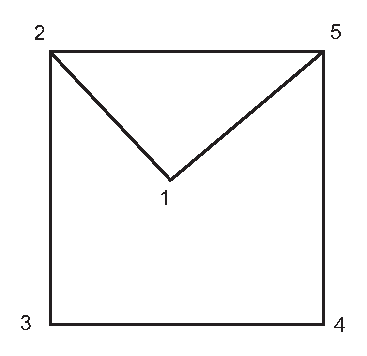
\includegraphics{\ps/no4circuit.eps}
  \caption{A node of type $(1,0,1)$, and a contour loop}
  \label{fig:no4circuit:bis}
\end{figure}

\begin{lemma}\label{lemma:nobad4}
Let $(H,\azim,\flat,\sigma)$ be a formally contravening hypermap.
Let $v$ be a node of type $(1,0,1)$ with precisely one triangle and
one pentagon, as show in Figure~\ref{fig:no4circuit:bis}. Let $L$ be
the perimeter contour loop with four face steps having the node $v$
in its interior.  At each of the four nodes $w$ visited by $L$, let
$\azim(w)$ be the sum of the terms $\azim(x)$, with the sum running
over the darts $x$ at the node visited by $L$.  Then
    $\azim(w) > 1.32$
for each of the four nodes $w$ visited by $L$.
\end{lemma}

\begin{lemma} Let $(H,\azim,\flat,\sigma)$ be a formally contravening
hypermap.  Let $v$ be a node of $H$ of type $(1,0,1)$, such that the
exceptional region is a pentagon.  Let $W$ be the set of four nodes
of the pentagon other than $v$.  If there are four triangles
$F_1,\ldots,F_4$ at some node $W$ that do not meet $v$, then
    $$\sum_{i=1}^p \tau(F_i) > a(4)\,\pt.$$
\end{lemma}

\begin{lemma}
Let $(H,\azim,\flat,\sigma)$ be a formally contravening hypermap.
Let $X$ be the set of nodes $v$ with the following properties.
    \begin{enumerate}
    \item The node has type $(5,0,1)$.
    \item The exceptional face at the node is pentagonal.
    \item That pentagonal face has no nodes of type $(1,0,1)$.
    \end{enumerate}
Then $\card(X)\ne 1$.
\end{lemma}

\begin{lemma}  Let $(H,\azim,\flat,\sigma)$ be a formally contravening
hypermap.  If $F$ is a face of cardinality $3$ or $4$, and if $x$ is
a dart of $F$, then $\tau(F),\sigma(F),\azim(x)$ satisfy the linear
constraints marked {``assumed conditions''} in the linear program of
Section~\ref{sec:ccc}.
\end{lemma}

\begin{lemma} Let $(H,\azim,\flat,\sigma)$ be a formally contravening
hypermap.  The function $\flat$ has the following properties.
    \begin{itemize}
    \item $\flat$ is a boolean-valued function, whose
     domain is the set of darts in exceptional faces of
    $H$.
    \item If $\azim(x)\le 1.32$, then $\flat(x)$.
    \end{itemize}
\end{lemma}

\begin{lemma}  Let $(H,\azim,\flat,\sigma)$ be a formally contravening
hypermap. Assume that $v$ is a node of $H$ whose type is
$(p,q,r)=(3,0,2)$ or $(4,0,1)$.  Assume that $\neg\flat(x)$ for
every dart of $v$.  Let $\tau(F_1),\ldots,\tau(F_p)$ be the
triangles at the node $v$.  Then
    $$
    \sum_{i=1}^p \tau(F_i) > a(p)\,\pt.
    $$
\end{lemma}



\chapter{Formal Contravention is Tame}
    \label{sec:contraproof}

This section begins the proof of Theorem~\ref{theorem:contravene}
(formally contravening hypermaps are tame). To prove Theorem
\ref{theorem:contravene}, it is enough to show that each defining
property of tameness is satisfied for every formally contravening
hypermap. This is the substance of results in the following
sections. The proof continues through the end of
\Chap~\ref{sec:weight}. This chapter verifies all the properties of
tameness, except for the last one (weight assignments).

\section{First Properties}

This section verifies the first XX properties of tameness.  Note
that the properties XX - XXX all hold by Lemma~\ref{XX}.

[XX Move to hypermap section:]

\begin{lemma} Let $(D,e,n,f)$ be a plane hypermap such that every face has
cardinality at least $3$ and no face meets a node in more than one
dart.  Then no dart is a fixed point under $n$.
\end{lemma}

\begin{proof}  Let $x$ be a fixed point under
$n$. We claim that $e x$ and $f x$ lie on the same node and the same
face, so are equal by Lemma~XX.  They are on the same node because
$n(f x) = e^{-1} x = e x$. They are on the same face because
    $$f^2 (e x) =  f(n^{-1} x) = f x.$$
So $e x = f x$.   Thus, $f^2 (e x) = f x = e x$, so $e x$ lies on a
face of cardinality at most two.  This contradicts an assumption.
\end{proof}


\begin{lemma} Formally contravening hypermaps satisfy Property
\ref{definition:tame:degree} of tameness: The cardinality of every
node is at least $2$ and at most $6$.
\end{lemma}

\begin{proof}  A node of cardinality one is a dart
$x$ that is the fixed point of $n$.

Let the type of the node be $(p,q,r)$.  If $r=0$, then the
impossibility of a node of cardinality $7$ or more is found in the
table entry $b(7,0)$ (Lemma~\ref{lemma:pq-types:bis}). If $r\ge1$,
then Lemma~\ref{lemma:0.8638} shows that the azimuth angles of the
darts at the node cannot sum to $2\pi$:
    $$6 (0.8638) + 1.153 > 2\pi.$$
\end{proof}



\section{Computer Calculations and Their Consequences}
\label{sec:ccc}

We have the following linear program. There are many different
choices of objective function and constraint {\it Csum} depending on
the particular constants $\sLP$, $\tauLP$, or $\tlp/\pt$ that need
to be computed.  In the linear program the constants $\pi$ and $\pt$
are replaced by numerical approximations.  Section~\ref{XX} explains
how the output from the numerical routines can be adjusted to yield
perfectly rigorous results.  The listing is in a format that can be
read by the program {\it LPSolve}.  See \cite{lpsolve}.

The origin of these inequalities is interval arithmetic.  They are
listed in nonlinear form at \cite{XX}.  The numeric labels of the
equations here is consistent with the labels in that archive.

The correspondence between linear program variables in the program
listing and the variables in use elsewhere in the book is the
following.  Here $F$ is a face, and $x$ is a dart in that face.
    $$
    \begin{array}{lll}
    \card(F)=3 &\Rightarrow\  \azim(x)=\azim_3,\ \tau(F)=\op{tau}_3,\ \sigma(F)=\op{sigma}_3\\
    \card(F)=4 &\Rightarrow\  \azim(x)=\azim_4,\ \tau(F)=\op{tau}_4,\ \sigma(F)=\op{sigma}_4\\
    \end{array}
    $$

{ \obeylines\tt
  \hbox{}\parindent=4pt

 /* Change  "min/max" and "Csum", according to the objective */
 \ \hbox{}
 /* This example computes b(2,2) */
 // min: 2 tau3\_s + 2 tau4\_s;
 // Csum: 2 azim3 + 2 azim4 - twopi = 0;
 \ \hbox{}
 /* This example computes tauLP(2,2,5.0) */
 //min: 2 tau3 + 2 tau4;
 //Csum: 2 azim3 + 2 tau4 <= 5.0;
 \ \hbox{}
 /* This example computes sigmaLP(5,0,2pi-1.153) */
 max: 5 sigma3 + 0 sigma4;
 Csum: 5 azim3 + 0 sigma4 - twopi <= -1.153;
 \ \hbox{}
 /* Variable bounds */
 twopi: twopi =  6.2831853071795862;
 \ \hbox{}
 // pt = 0.055373645668464144;
 Ctaup: 0.055373645668464144 tau3\_s - tau3 = 0;
 Ctauq: 0.055373645668464144 tau4\_s - tau4 = 0;
 \ \hbox{}
 /* assumed conditions: */
 /* triangle tau */
 J927432550: 0.3897 azim3 + tau3 > 0.4666;
 J221945658: 0.2993 azim3 + tau3 > 0.3683;
 J53415898:  tau3 > 0.0;
 J106537269: -0.1689 azim3 + tau3 > -0.208;
 J254527291: -0.2529 azim3 + tau3 > -0.3442;
 \ \hbox{}
 /* triangle sigma */
 J539256862: sigma3 - 0.37898 azim3 < -0.4111;
 J864218323: sigma3 + 0.142 azim3 < 0.23021;
 Jsigma\_1pt: -Infinity <= sigma3 <= 1.0;
 J776305271: sigma3 + 0.3302 azim3 < 0.5353;
 \ \hbox{}
 /* quad  tau */
 J539320075: 4.49461 azim4 + tau4 > 5.81446 ;
 J122375455: 2.1406 azim4 + tau4 > 2.955;
 J408478278: 0.316 azim4 + tau4 > 0.6438;
 J996268658: tau4 > 0.1317;
 J393682353: -0.2365 azim4 + tau4 > -0.3825;
 J775642319: -0.4747 azim4 + tau4 > -1.071;
 \ \hbox{}
 /* quad sigma */
 J310151857: sigma4 - 4.56766 azim4 < -5.7906;
 J655029773: sigma4 - 1.5094 azim4 < -2.0749;
 J\_73283761:  sigma4 - 0.5301 azim4 < -0.8341;
 JLemm14\_11: -Infinity <= sigma4 <= 0;
 J\_15141595:  sigma4 - 0.3878 azim4 < -0.6284;
 J574391221: sigma4 + 0.1897 azim4 < 0.4124;
 J396281725: sigma4 + 0.5905 azim4 < 1.5707;
 \ \hbox{}

 /* all vars have lower bound 0, except sigma3, sigma4  */


}

\bigskip

We let $\tauLP(p,q,\alpha)$ denote the solution to this linear
program with objective $$\min: p\, \tau_3 + q\, \tau_4$$ and
constraint
$$\op{Csum}: p\, \azim_3 + q\,\azim_4 \le d.$$

We let $\tlp(p,q)$ denote the solution to this linear program with
objective $$\min: p \tau_3 + q \tau_4$$ and constraint
$$\op{Csum}: p\, \azim_3 + q\,\azim_4 =2\pi.$$  The constants $b(p,q)$
are computed as lower bounds satisfying $\tlp(p,q) > b(p,q)\,\pt$,
which the exception of the constants $b(5,0)$ and $b(7,0)$, which
are slight improvements on the linear programs.

We let $\sLP(p,q,\alpha)$ denote the solution to this linear program
with objective $$\max: p\, \sigma_3 + q\, \sigma_4$$ and constraint
$$\op{Csum}: p\, \azim_3 + q\,\azim_4 \le d.$$



\begin{lemma} We have the following estimates:
    $$
    \begin{array}{lll}
    &s_5+\sLP(5,0,2\pi-1.153)< c(8)\,\pt\\
    &s_6+\sLP(5,0,2\pi-1.153) < s_9\\
    &s_5+\sLP(5,0,2\pi-1.153)<s_8\\
    &(9-2(0.48))\,\pt+s_5+\sLP(2,2,2\pi-1.153)<8\,\pt\\
    &2t_5+\tauLP(4,0,2\pi-2(1.153))>\squander\\
    \end{array}
    $$
\end{lemma}

\begin{proof} Run the linear programs and see what you get.
\end{proof}

These are just a few of a long list of inequalities such as these
that will appear in the pages that follow.  They all come from the
same basic linear program with varying objective function and angle
sum constraint.

\section{Linear Programs} %subsection
\label{sec:2.2}  To continue with the proof that formally
contravening hypermaps are tame, we need to introduce some more
notation and methods.



\begin{lemma}
    A formally contravening hypermap satisfies
    Property \ref{definition:tame:score} of tameness:
    $$\sum_F c(\card(F)) \ge 8.$$
\end{lemma}

\begin{proof}  By Lemma~\ref{XX7.6},
We will show that
    \begin{equation}
    c(\card(F))\,\pt \ge s_n \ge \sigma(F)
    \label{eqn:sigma}
    \end{equation}
The result follows for formally contravening
    hypermaps:
    $$
    \begin{array}{lll}
        \sum_F c(\card(F)) \,\pt &\ge \sum_F \sigma(F) \\
            &= \sigma^*(H) \ge 8\,\pt.
    \end{array}
    $$
\end{proof}

\begin{lemma}
    \label{proposition:wttau}
    Let $F$ be a face of a formally contravening hypermap.
    Then
    $$\tau(F) \ge d(\card(F))\pt.$$
\end{lemma}

\begin{proof} Similar.
\end{proof}

\begin{lemma}  If $v$  is a node of an exceptional face,
and if there are $6$ faces meeting at $v$, then the exceptional face
is a pentagon and the other $5$ faces are triangles.  In particular,
the node has type $(5,0,1)$.
\end{lemma}

\begin{proof}  Let $(p,q,r)$ be the type of the node.  We consider
several cases, according to the value of $p$.

{\bf($p\le2$)} If there are at least four non-triangular regions at
the node, then the sum of azimuth angles around the node is at least
$4(1.153)+2(0.8638)>2\pi$, which is impossible.  (See
Lemma~\ref{lemma:0.8638}.)

{\bf($p=3$)} If there are three non-triangular regions at the node,
then $\tau^*(H)$ is at least
$2t_4+t_5+\tauLP(3,0,2\pi-3(1.153))>\squander$.

{\bf($p=4$)} If there are two exceptional regions at the node, then
$\tau^*(H)$ is at least $2t_5+\tauLP(4,0,2\pi-2(1.153))>\squander$.

If there are two non-triangular regions at the node, then
$\tau^*(H)$ is at least  $t_5+\tauLP(4,1,2\pi-1.153)>\squander$.

{\bf($p=5$)} We are left with the case of five triangles and one
exceptional face.

When there is an exceptional face at a node of cardinality six, we
claim that the exceptional face must be a pentagon. If the face is a
heptagon or more, then $\tau^*(H)$ is at least
$t_7+\tauLP(5,0,2\pi-1.153) > \squander$.

If the face is a hexagon, then $\tau^*(H)$ is at least $t_6 +
\tauLP(5,0,2\pi-1.153) > t_9$. Also, $s_6+\sLP(5,0,2\pi-1.153) <
s_9$. The contour loop around the six faces has at most $9$ face
steps. Lemma~\ref{lemma:s9-t9:bis} gives the bound of $8\,\pt$.
\end{proof}


\begin{lemma}
    \label{lemma:aggregate6}
    Let $(H,\azim,\flat,\sigma)$ be formally contravening.
    \begin{enumerate}
    \item The aggregate $F$ of the six faces at a node of type
    $(5,0,1)$ satisfies
            $$
            \begin{array}{lll}
            \sigma(F) < s_8,\\
            \tau(F) > t_8.
            \end{array}
            $$
    \item There are at most two nodes of type $(5,0,1)$.  If
        there are two, then they are non-adjacent vertices on a
        pentagon, as shown in Figure \ref{fig:doubledegree6}.  (The
        pentagon has a node of type $(1,0,1)$.)
    \end{enumerate}
\end{lemma}
\begin{figure}[htb]
  \centering
  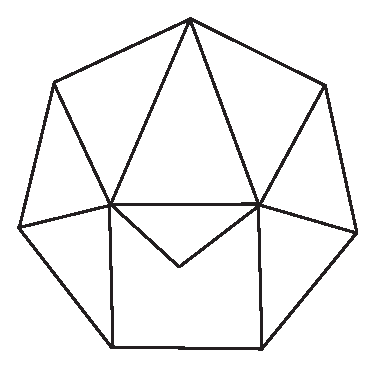
\includegraphics{\ps/doubledegree6.eps}
  \caption{Non-adjacent nodes of cardinality $6$ on a pentagon}
  \label{fig:doubledegree6}
\end{figure}

\begin{proof}
We begin with the first part of the lemma. The sum  $\tau(F)$ over
these six standard regions is at least
    $$t_5+\tauLP(5,0,2\pi-1.153)> t_8.$$
Similarly,
    $$s_5+\sLP(5,0,2\pi-1.153)<s_8.$$
%
We note that there can be at most one exceptional face with a node
of cardinality six.  Indeed, if there are two, then they must both
be nodes of the same pentagon:
    $$t_8+t_5>\squander.$$
Such a second node on the octagonal aggregate leads to one of the
follow constants greater than $\squander$.  These same constants
show that such a second node on a hexagonal aggregate must share two
triangular faces with the first node of cardinality six.
$$\begin{array}{lll}
    t_8 &+\tauLP(4,0,2\pi-1.32-0.8638),\quad\text{or}\\
    t_8 &+1.47\,\pt+\tauLP(4,0,2\pi-1.153-0.8638),\quad\text{or}\\
    t_8 &+\tauLP(5,0,2\pi-1.153) .
\end{array}
$$
(The relevant constants are found at Lemma~\ref{lemma:1.47} and
Lemma~\ref{lemma:0.8638}.)
\end{proof}

\section{An impossible node}
\label{sec:impossible}

This subsection rules out the existence of nodes of type $(1,0,1)$,
where the exceptional face is a pentagon.  The node and its
surrounding contour loop are show in Figure~\ref{fig:no4circuit:bis}
with nodes marked $v_1,\ldots,v_5$. The node $v_1$ is the interior
node, the triangle is $(v_1,v_2,v_5)$ and the pentagon is
$(v_1,\ldots,v_5)$. Two of the assumptions (XX and XX) relate to
this node.

\begin{lemma}\label{lemma:nobad4}
No formally contravening hypermap contains this configuration.
\end{lemma}

\begin{proof}
Let $F_3$ and $F_5$ be the triangle and pentagon, respectively. By
Lemma~\ref{lemma:11.16:bis}, we have
    $$\tau(F_3)+\tau(F_5)\ge 11.16\,\pt.$$
There are no other exceptional faces, because
$11.16\,\pt+t_5>\squander$. Every node not meeting $F_3\cup F_5$ has
type $(5,0,0)$, by Lemma~\ref{lemma:pq:bis}. In particular, there
are no quadrilateral regions.  By Lemma~\ref{lemma:nobad4}, the sum
of the azimuth angles at a node meeting $F_3\cup F_5$ is at least
$1.32$. There are at most $4$ triangles at every vertex of $P$,
because
    $$
    11.16\,\pt+\tauLP(5,0,2\pi-1.32)>\squander.
    $$
    %6.02\,\pt$.
There are at least $3$ triangles besides $F_3$ at every node meeting
$F_3\cup F_5$ (except the node $v_1$), otherwise we contradict
Lemma~\ref{lemma:no-enclosed-tri:bis} or Lemma~\ref{lemma:no-2}.

The only triangulation with these properties is obtained by removing
one edge from the icosahedron.  (We leave this as a tedious
exercise.  Use face-insertion.) This implies that there are two
opposite nodes (either $(v_2,v_4)$ or $(v_3,v_5)$) each having four
triangles besides $F_3$.   Lemma~\ref{XXLast} show that the set $A$
of these eight triangles satisfies
    $$
    \sum_{F\in A} \tau(F) \ge 2(1.5)\,\pt.
    $$
An icosahedron has two additional nodes of type $(5,0,0)$ whose
triangles are distinct from the eight already mentioned.  They
contribute an additional $2(0.55)\,\pt$ to $\tau^*(H)$.   Now
$$\tau^*(H)\ge (11.16+2(1.5)+2(0.55))\,\pt>\squander$$ by
Lemma~\ref{lemma:0.55:bis}.   The result follows.
\end{proof}

\begin{lemma} \label{lemma:deg5}
Every formally contravening hypermap satisfies Property
\ref{definition:tame:degreeE} of tameness: If a node meets an
exceptional face, then the cardinality of the node is at most $5$.
\end{lemma}

\begin{proof} Every node of type $(5,0,1)$ meets a face that is a pentagon.
If there are two or more such nodes, then it must be that of Lemma
XX.  However, this has a node of type $(1,0,1)$, which is ruled out
by Lemma XX.  Thus, there is at most one node of type $(5,0,1)$.
This arrangement does not appear on a formally contravening hypermap
by Lemma~\ref{lemma:nobad4}.
\end{proof}



\section{Possible four-circuits}

Every contour loop partitions the faces into the interior and
exterior.  Every contour loop partitions the nodes that do not meet
the loop into exterior and interior nodes.
%
 \index{interior node}

Lemma~\ref{lemma:no-2} asserts that either the interior or the
exterior has at most $1$ enclosed vertex.   When choosing which
aggregate is to be called the interior, we may make our choice so
that the interior has area at most $2\pi$, and hence contains at
most $1$ node. With this choice, we have the following lemma.

\begin{lemma}
Let $(H,\azim,\flat,\sigma)$ be a formally contravening hypermap. If
$L$ is a contour loop with $4$ face steps, and there are at least
two nodes in the exterior of $L$, then the interior of $L$ takes one
of the forms illustrated in Figure XX in Property
    \ref{definition:tame:4-circuit} of tameness.
\end{lemma}

\begin{proof}
By Lemma~XX, the interior of $L$ contains at most one node.

$H$ is a connected plane planar map.  We form a normal family of
contour loops ${\cal L}$ by taking the contour loop $L^{-1}$
reversing $L$ (XX explain) and all the faces in the interior of $L$.
(Check this is a normal family.)  The quotient $H' = H/{\cal L}$ is
a plane planar map.  There is a further quotient of $H'$ with normal
family $\{L,L^{-1}\}$, which is isomorphic to $P_4$ with the natural
flag coming from $H'$.  The niceness conditions of LemmaXX are
satisfied, so we can recover $H'$ from $P_4$ by a sequence of
face-insertions.  Since the interior of $L$ contains at most one
node, this gives restrictions on the partitions that can be used in
face-insertion.

If there are no enclosed vertices, then the only possibilities are
for it to be a single quadrilateral face or a pair of adjacent
triangles.

Assume there is one enclosed vertex $v$.  If $v$ is connected to $3$
or $4$ nodes of the quadrilateral, then that possibility is listed
as part of the conclusion.

If $v$ is connected to $2$ opposite nodes in the $4$-cycle, then the
node $v$ has type $(0,2,0)$ and the bounds of
Lemma~\ref{lemma:pq:bis} show that the hypermap cannot be formally
contravening.

If $v$ is connected to $2$ adjacent nodes in the $4$-cycle, then we
appeal to Lemma~\ref{lemma:nobad4} to conclude that the hypermap
does not contravene.

If $v$ is connected to $0$ or $1$ nodes, then we appeal to
Lemma~\ref{lemma:enclosed:bis}.  This completes the proof.
\end{proof}

\section{Weight Assignments}
    \label{sec:weight}

The purpose of this section is to prove the existence of a good
admissible weight assignment for formally contravening hypermaps.
This will complete the proof that all formally contravening
hypermaps are tame.

\begin{theorem}  Every formally contravening hypermap has an admissible
weight assignment of total weight less than $\op{tgt}=14.8$.
\end{theorem}

Given a formally contravening hypermap $(H,\azim,\flat,\sigma)$, we
define a weight assignment $w$ by
    $$F \mapsto w(F) = \tau(F)/\pt.$$
Since the hypermap is formally contravening,
    $$
    \begin{array}{lll}
    \sum_F w(F) &= \sum_F \tau(F)/\pt \\
            &= \tau^*(H)/\pt\,\le\,\squander/\pt \\
        &< \op{tgt}=14.8.
    \end{array}
    $$
The challenge of the theorem will be to prove that $w$, when
defined by this formula, is admissible.

\section{Admissibility}
\label{sec:admissibility}

The next three lemmas establish that this definition of $w(F)$ for
formally contravening hypermaps satisfies the first three defining
properties of an admissible weight assignment.

\begin{lemma}  Let $F$ be a face of cardinality $n$ in a formally contravening hypermap.
Define $w(F)$ as above. Then
        $w(F) \ge d(n)$.
\end{lemma}

\begin{proof} This is Lemma~\ref{proposition:wttau}.
\end{proof}

\begin{lemma} Let $v$ be a node of type $(p,q,0)$ in a
formally contravening hypermap.  Define $w(F)$ as above. Then
        $$\sum_{v\in F} w(F) \ge b(p,q).$$
\end{lemma}


\begin{proof} This is Lemma~\ref{lemma:pq:bis}.
\end{proof}

\begin{lemma} Let $V$ be any set of nodes of type $(5,0,0)$ in a
formally contravening hypermap.  Define $w(F)$ as above.
        If the cardinality of $V$ is $k\le 4$,
        then
        $$\sum_{V\cap F\ne\emptyset} w(F) \ge 0.55 k.$$
\end{lemma}

\begin{proof} This is Lemma~\ref{lemma:0.55:bis}.
\end{proof}

The following theorem establishes the final property that $w(F)$
must satisfy to make it admissible.  {\it Separated sets\/} are
defined in Section~\ref{sec:wtassign}.

\begin{theorem}
        \label{proposition:excess}
        Let $V$ be any separated set of nodes in a formally contravening hypermap.
        Define $w(F)$ as above.
        Then
        $$\sum_{V\cap F\ne\emptyset} (w(F) -d(\card(F)))
            \ge \sum_{v\in V} a(p_v),$$
        where $p_v$ denotes the number of triangles containing
        the node $v$.
\end{theorem}

The proof will occupy the rest of this \chap. Since the cardinality
of each node is five, and there is at least one face that is not a
triangle at the node, the only constants $p_v$ that arise are
    $$p_v \in\{0,\ldots,4\}$$
We will prove that in a formally contravening hypermap that the
Properties (1) and (4) of a separated set are incompatible with
$p_v\le 2$.  This will allows us to assume that
$$p_v\in\{3,4\},$$ for all $v\in V$.  These cases will be treated in
Section~\ref{sec:tri34}.

\section{Proof that $p_v>2$}
%subsection
\label{sec:2.4} \label{sec:tri2}

In this subsection $(H,\azim,\flat,\sigma)$ is a formally
contravening hypermap.  Let $V$ be a separated set of nodes in $H$.

\begin{lemma}  Under these conditions, for every $v\in V$,
$p_v>1$.
\end{lemma}

\begin{proof}
If there are $p$ triangles, $q$ quadrilaterals, and $r$ other
faces, then
    $$
    \begin{array}{lll}
    \tau^*(H) &\ge\sum_{v\in F}\tau(F)\\
        &\ge r\, t_5 + \tauLP(p,q,2\pi-r(1.153)).
    \end{array}
    $$ If there is a node $w$ that is
not on any of the faces containing $v$, then the sum of $\tau(F)$
over the faces containing $w$ yield an additional $0.55\,\pt$ by
Lemma~\ref{lemma:0.55:bis}. We calculate these constants for each
$(p,q,r)$ and find that the bound is always greater than
$\squander$. This implies that $H$ cannot be formally contravening.
$$\begin{array}{llll}
    (p,q,r)&\hbox{\it lower bound }&\hbox{\it justification}\\
    &\\
    (0,5,0)&22.27\,\pt&\text{Lemma~\ref{lemma:pq:bis}}\\
    (0,q,r\ge1)& t_5+4 t_4\approx 14.41\,\pt +0.55\,\pt& \\
    (1,4,0) &17.62\,\pt &\text{Lemma~\ref{lemma:pq:bis}}\\
    (1,3,1) &t_5 + 12.58\,\pt &(\tauLP)\\
    (1,2,2) &2t_5 + 7.53\,\pt &(\tauLP)\\
    (1,q,r\ge3)& 3 t_5 + t_4& \\
\end{array}
$$
\end{proof}


\begin{lemma} Under these same conditions, for every $v\in V$,
$p_v>2$.
\end{lemma}

\begin{proof}
Assume that $p_v=2$.  We will show that this implies that $H$ does
not contravene.  Let $r=r_v$ be the number of exceptional faces at
$v$. We have $r+p_v\le5$.  We consider various cases, according to
the value of $r$.

The constants $0.55\,\pt$ and $0.48\,\pt$ used throughout the
proof come from Lemma~\ref{lemma:0.55:bis}. The constants $t_n$
comes from Lemma~\ref{lemma:sn-tn}.

($(p,q,r)=(2,0,3)$): First, assume that there are three exceptional
faces around node $v$. They must all be pentagons
($2t_5+t_6>\squander$). The aggregate of the five faces is an
$m$-gon (some $m\le11$).  If there is a node not on this aggregate,
use $3t_5+0.55\,\pt>\squander$. So there are at most nine triangles
away from the aggregate, and the Euler relation gives
    $$
    \sigma^*(H) \le 9\,\pt + (3 s_5+2\,\pt) < 8\,\pt.
    $$

($(p,q,r)=(2,1,2)$): The argument if there is a quad, pentagon, and
hexagon is the same $(t_4+t_6=2t_5,s_4+s_6=2s_5)$.

Assume next that there are two pentagons and a quadrilateral around
the node. The contour loop around the two pentagons, quadrilateral,
and two triangles is has $m$ face steps (some $m\le10$). There must
be a node exterior to this loop, for otherwise the Euler relation
gives
    $$
    \sigma^*(H) \le 8\,\pt+(2s_5+2\,\pt)<8\,\pt.
    $$

The azimuth angle of one of the pentagons is at most $1.32$.  For
otherwise, $\tauLP(2,1,2\pi-2(1.32))+2t_5+0.55\,\pt>\squander$.

Lemma~\ref{lemma:1.47} shows that any pentagon $F$ with an azimuth
angle less than $1.32$ yields $\tau(F)\ge t_5+ (1.47\,\pt)$. If both
pentagons have an azimuth angle $<1.32$ the lemma follows easily
from this calculation:
    $2(t_5+1.47\,\pt)\,\pt+\tauLP(2,1,2\pi-2(1.153))+0.55\,\pt>\squander$.
If there is one pentagon with angle $>1.32$, we then have
    $t_5+(1.47\,\pt)+\tauLP(2,1,2\pi-1.153-1.32)+t_5+0.55\,\pt>\squander$.


($(p,q,r)=(2,2,1)$): Assume finally that there is one exceptional
face at the node. If it is a hexagon (or more), we are done
$t_6+\tauLP(2,2,2\pi-1.153)>\squander$. Assume it is a pentagon. The
contour loop around the five faces at the node has $m$ face steps
(some $m\le9$). If there are no more than $9$ triangles exterior to
the contour loop, then $\sigma^*(H)$ is at most
$(9-2(0.48))\,\pt+s_5+\sLP(2,2,2\pi-1.153)<8\,\pt$
(Lemma~\ref{lemma:0.55:bis}). So by the Euler relation, we may
assume that there are at least three nodes exterior to the contour
loop.

If the azimuth angle of the dart on the pentagon is greater than
$1.32$, we have
  $$\tau^*(H)\ge\tauLP(2,2,2\pi-1.32) +3(0.55)\,\pt +t_5 > \squander;$$
and if it is less than $1.32$, we have by Lemma~\ref{lemma:1.47}
    $$
    \begin{array}{lll}
        \tau^*(H)\ge\tauLP(2,2,2\pi-1.153)&+3(0.55)\pt+1.47\,\pt+t_5 \\
            &> \squander.
    \end{array}
    $$
\end{proof}

\section{Bounds when $p_v\in\{3,4\}$.  } %subsection
\label{sec:2.7} \label{sec:tri34}

In this subsection $(H,\azim,\flat,\sigma)$ is a formally
contravening hypermap.  Let $V$ be a separated set of nodes.  We
assume that there are three or four triangles meeting $v$, for every
$v\in V$.

To prove the Inequality \ref{definition:admissible:excess} in the
definition of admissible weight assignments, we will rely on the
following reductions. Define an equivalence relation on exceptional
faces by $F\sim F'$ if $F=F'$ or if there is a sequence
$F=F_0,\ldots, F_r=F'$ of exceptional faces such that consecutive
faces share a node of type $(3,0,2)$. Let ${\cal F}$ be an
equivalence class of faces.

%% XX GIVE FIGURE HERE with lots of exceptionals.

\begin{lemma} Let $V$ be a separated set of nodes.  For every
equivalence class of exceptional faces $\cal F$, let $V({\cal F})$
be the subset of $V$ whose nodes meet a face in ${\cal F}$. Suppose
that for every equivalence class $\cal F$, the Inequality
\ref{definition:admissible:excess} (in the definition of admissible
weight assignments) holds for $V({\cal F})$. Then the Inequality
holds for $V$.
\end{lemma}

\begin{proof}
By construction, each node in $V$ lies in some $F$, for an
exceptional face.  Moreover, the separating property of $V$ insures
that the triangles and quadrilaterals in the inequality are
associated with a well-defined  ${\cal F}$. Thus, the inequality for
$V$ is a sum of the inequalities for each $V({\cal F})$.
\end{proof}


\begin{lemma}
\label{lemma:split}
 Let $v$ be a node of type $(p,q,r)$ in a separated set $V$.  Suppose that
for some $p'\le p$ and $q'\le q$, we have
    $$\tauLP(p',q',\alpha) \ge ( p' d(3) + q' d(4) + a(p))\,\pt$$
for some upper bound $\alpha$ on the angle occupied by $p'$
triangles and $q'$ quadrilaterals at $v$.  Suppose further that the
Inequality~\ref{definition:admissible:excess} (in REFXX) holds for
the separated set $V' = V\setminus \{v\}$. Then the inequality holds
for $V$.
\end{lemma}

\begin{proof}  Let $F_1,\ldots,F_m$, $m={p'+q'}$, be faces corresponding
to the triangles and quadrilaterals in the lemma.  The hypotheses
of the lemma imply that
    $$\sum_{1}^{m} (w(F_i) - d(\card(F_i))) \ge a(p).$$
Clearly, the Inequality for $V$ is the sum of this inequality, the
inequality for $V'$, and $w(F)- d(F)\ge0$.
\end{proof}








\begin{lemma}  Property \ref{definition:admissible:excess}  of
admissibility holds.  That is, let $V$ be any separated set of
nodes. Then
        $$\sum_{F:\,V\cap F\ne\emptyset} (w(F) -d(\card(F)))
            \ge \sum_{v\in V} a(p_v).$$
\end{lemma}

\begin{proof}  Let $V$ be a separated set of nodes.
The results of Section~\ref{sec:tri2} reduce the lemma to the case
where $p_v\in\{3,4\}$ for every node $v\in V$.


One case is easy to deal with.  Assume the node has type $(3,1,1)$.
 Assume the azimuth angle of the dart on the exceptional face is
least $1.32$, then
    \begin{equation}
    \tauLP(3,1,2\pi-1.32)>1.4\,\pt + t_4.
    \label{eqn:tau1.32}
    \end{equation}
This gives the bound in the sense of Lemma~\ref{lemma:split} at such
a node. For the rest of the proof, assume that the azimuth angle on
the exceptional face $F$ is less than $1.32$ at nodes of type
$(p,q,r)=(3,1,1)$. This implies in particular by
Lemma~\ref{lemma:1.32:bis} that the dart $x(F,v)$ is flat.

Let $v$ be node with no flat darts.   By Lemma~\ref{lemma:1.32:bis},
the azimuth angles of the
exceptional regions at $v$ are at least $1.32$.   It follows%
%\footnote{\calc{551665569}, \calc{824762926}, and
%\calc{325738864}}
%% K.C.-2002-version: 17.20 Group 20, 17.21 Group 21. (page 49).
from Lemma~\ref{XX} that
    \begin{equation}
    \tauLP(p_v,q_v,\alpha) > ( p_v d(3) + q_v d(4) + a(p_v))\,\pt.
    \label{eqn:tau-alpha}
    \end{equation}
Thus, by Lemma~\ref{lemma:split}, we reduce to the case where for
each $v\in V$,  there is flat dart at $v$.  Assume that $V$ has this
property.

Pick a function $f$ from the set $V$ to the set of exceptional
standard regions as follows. Let $X$ be the set of exceptional faces
$F$ at $v$ for which $x(F,v)$ is flat.  From $X$, let $f(v)$ be the
one with smallest $\azim(x(F,v))$.  We see by construction and
Lemma~\ref{lemma:1.32:bis} that $F = f(v)$ has the properties:
    \begin{itemize}
        \item $\flat(x(F,v))$
        \item $\azim(x(F,v)) > 1.32\ \Rightarrow\ \azim(x(F',v)) >
        1.32$, for any exceptional face $F'$ meeting $v$.
    \end{itemize}

For each exceptional face $F$, let
    $$V_F = \{ v\in V : f(v) = F\}.$$  This set may be empty for
some $F$.  Let $A_F$ be the union of $\{F\}$, and the set of
triangles and quadrilaterals with a dart in some $v\in V_F$.  If
$V_F$ is empty, then $A_F =\{F\}$.  The indexing set $A$ of Property
\ref{definition:admissible:excess} of admissibility is the disjoint
union of $A_F$.  The set $V$ is the disjoint union of the $V_F$ (or
at least of the nonempty ones). So the result follows from
Lemma~\ref{XX} for all the faces.
\end{proof}



The proof that formally contravening hypermaps are tame is complete.
